\documentclass[11pt]{ctexart}
\usepackage[a4paper,margin=2.4cm]{geometry}
\usepackage{graphicx}
\usepackage{amsmath}
\usepackage{amssymb}
\usepackage{listings}
\usepackage{xcolor}
\usepackage{booktabs}
\usepackage{float}
\usepackage{caption}
\usepackage{subcaption}
\usepackage{enumitem}
\usepackage[hidelinks]{hyperref}

% 中文字体（系统已确认存在 Noto CJK）
\setCJKmainfont{Noto Serif CJK SC}
\setCJKsansfont{Noto Sans CJK SC}
\setCJKmonofont{Noto Sans Mono CJK SC}

\captionsetup{font=small,labelfont=bf}

\definecolor{codebg}{RGB}{246,247,249}
\definecolor{codekw}{RGB}{30,80,170}
\definecolor{codecm}{RGB}{60,130,70}
\definecolor{codestr}{RGB}{190,110,30}

\lstdefinestyle{cpp}{
  language=C++,
  basicstyle=\ttfamily\small,
  keywordstyle=\color{codekw}\bfseries,
  commentstyle=\color{codecm}\itshape,
  stringstyle=\color{codestr},
  numbers=left,
  numberstyle=\tiny\color{gray},
  numbersep=8pt,
  frame=single,
  framerule=0.4pt,
  rulecolor=\color{gray!55},
  backgroundcolor=\color{codebg},
  breaklines=true,
  showstringspaces=false,
  tabsize=2,
  columns=fullflexible,
  xleftmargin=16pt,
  aboveskip=8pt,
  belowskip=6pt,
}
\lstset{style=cpp}

\title{\textbf{光线追踪大作业实验报告}\\[4pt]\large 基础光线生成与 BVH 加速渲染}
\author{姓名：\underline{\hspace{3em}}\qquad 学号：\underline{\hspace{5em}}}
\date{\today}

\begin{document}
\maketitle

\begin{abstract}
\noindent 本次大作业基于课程提供的 C++ 光线追踪框架，完成了一个 Whitted 风格的光线追踪渲染器。
具体实现了四个核心函数：\texttt{Renderer::Render}（主光线生成）、\texttt{Triangle::getIntersection}
（光线–三角形求交，Möller–Trumbore 算法）、\texttt{Bounds3::IntersectP}（光线–包围盒求交，slab 测试）
与 \texttt{BVHAccel::getIntersection}（BVH 层次遍历加速求交）；并额外完成了 \texttt{Scene::castRay\_noBVH}
中的完整着色模型（加分项）。在 $1280\times960$ 分辨率、含 \textbf{4968} 个三角形的 Stanford Bunny 场景下，
BVH 模式约 \textbf{0.45\,s} 即可渲染出正确的着色图像。本文逐一说明各函数的算法原理、关键代码与实验结果。
\end{abstract}

\section{概述}

光线追踪通过\textbf{逆向}追踪从相机出发、穿过每个像素射入场景的光线，求出光线与场景的最近交点并在该点着色，
从而生成图像。当场景中三角形数量较大时，"对每条光线遍历所有三角形" 的暴力做法效率极低；为此需要使用
\textbf{层次包围盒（Bounding Volume Hierarchy, BVH）}对求交过程进行加速：先用廉价的光线–包围盒测试快速
排除大片不可能相交的空间，再递归深入到真正可能相交的少数三角形。整体渲染流程如图~\ref{fig:pipeline} 所示。

\begin{figure}[H]
  \centering
  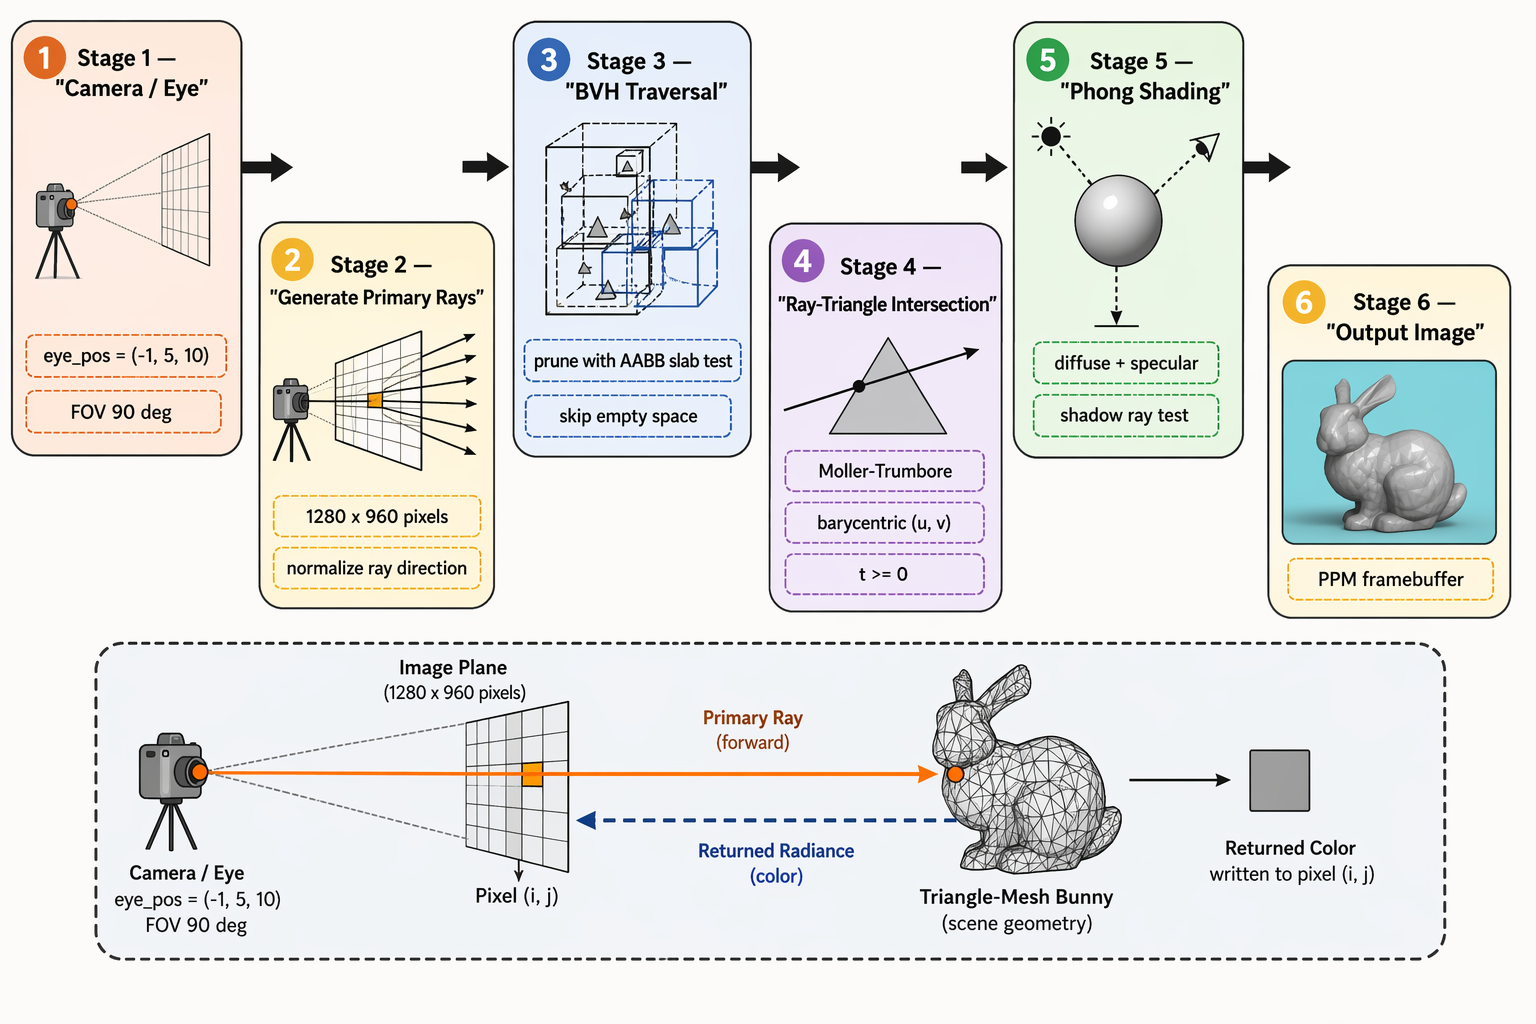
\includegraphics[width=\textwidth]{figures/pipeline.png}
  \caption{光线追踪渲染流程：相机生成主光线 $\rightarrow$ BVH 遍历剪枝 $\rightarrow$ Möller–Trumbore
  光线–三角形求交 $\rightarrow$ Phong 着色（含阴影测试）$\rightarrow$ 写入帧缓冲并输出 PPM 图像。}
  \label{fig:pipeline}
\end{figure}

本框架需要在以下文件中补全代码：\texttt{Renderer.cpp}、\texttt{Triangle.hpp}、\texttt{Bounds3.hpp}、
\texttt{BVH.cpp}，并可选地在 \texttt{Scene.cpp} 中补全着色模型。下面分别说明。

\section{各函数的实现}

\subsection{主光线生成：\texttt{Renderer::Render}}

该函数遍历图像的每个像素 $(i,j)$，构造一条从相机出发、穿过该像素中心的光线。设视场角为 \texttt{fov}，
则 $\text{scale}=\tan(\text{fov}/2)$，图像宽高比 $\text{aspect}=\text{width}/\text{height}$。
将像素坐标映射到位于 $z=-1$ 平面上的相机空间坐标：
\begin{align}
x &= \bigl(2\cdot\tfrac{i+0.5}{\text{width}}-1\bigr)\cdot\text{aspect}\cdot\text{scale},\\
y &= \bigl(1-2\cdot\tfrac{j+0.5}{\text{height}}\bigr)\cdot\text{scale}.
\end{align}
其中 $+0.5$ 使光线穿过像素中心，$y$ 方向取负是因为图像行号自上而下增大而相机 $y$ 轴向上。
随后归一化方向并投射光线：

\begin{lstlisting}
float x = (2.0f * (i + 0.5f) / scene.width  - 1.0f) * imageAspectRatio * scale;
float y = (1.0f - 2.0f * (j + 0.5f) / scene.height) * scale;
Vector3f dir = normalize(Vector3f(x, y, -1));
Ray ray(eye_pos, dir);
framebuffer[m++] = check_mode ? scene.castRay_noBVH(ray, 0) : scene.castRay(ray, 0);
\end{lstlisting}

最终把浮点颜色 \texttt{clamp} 到 $[0,1]$ 并按 P6 格式写出 \texttt{binary.ppm}。

\subsection{光线–三角形求交：\texttt{Triangle::getIntersection}（Möller–Trumbore）}

光线 $\mathbf{O}+t\mathbf{D}$ 与三角形 $(\mathbf{P}_0,\mathbf{P}_1,\mathbf{P}_2)$ 的交点可用重心坐标 $(u,v)$ 表示：
\begin{equation}
\mathbf{O}+t\mathbf{D}=(1-u-v)\mathbf{P}_0+u\mathbf{P}_1+v\mathbf{P}_2.
\end{equation}
令 $\mathbf{E}_1=\mathbf{P}_1-\mathbf{P}_0,\ \mathbf{E}_2=\mathbf{P}_2-\mathbf{P}_0,\ \mathbf{T}=\mathbf{O}-\mathbf{P}_0$，
由 Cramer 法则（Möller–Trumbore）可得
\begin{equation}
\begin{bmatrix}t\\u\\v\end{bmatrix}
=\frac{1}{\mathbf{E}_1\cdot(\mathbf{D}\times\mathbf{E}_2)}
\begin{bmatrix}
\mathbf{E}_2\cdot(\mathbf{T}\times\mathbf{E}_1)\\
\mathbf{T}\cdot(\mathbf{D}\times\mathbf{E}_2)\\
\mathbf{D}\cdot(\mathbf{T}\times\mathbf{E}_1)
\end{bmatrix}.
\end{equation}
有效交点必须满足 $u\ge0,\ v\ge0,\ u+v\le1$（落在三角形内）且 $t\ge0$（位于光线前方）。实现上：

\begin{lstlisting}
// 背面剔除：只对正对相机的面求交，避免封闭网格内壁干扰
if (dotProduct(ray.direction, normal) > 0) return inter;

Vector3f pvec = crossProduct(ray.direction, e2);
float det = dotProduct(e1, pvec);
if (fabs(det) < EPSILON) return inter;          // 光线与三角形平行

float invDet = 1.0f / det;
Vector3f tvec = ray.origin - v0;
float u = dotProduct(tvec, pvec) * invDet;
if (u < 0 || u > 1) return inter;
Vector3f qvec = crossProduct(tvec, e1);
float v = dotProduct(ray.direction, qvec) * invDet;
if (v < 0 || u + v > 1) return inter;
float t = dotProduct(e2, qvec) * invDet;
if (t < 0) return inter;                         // 交点在光线起点之后

inter.happened = true;  inter.coords = ray(t);
inter.normal = normal;  inter.distance = t;
inter.obj = this;       inter.m = m;
\end{lstlisting}

\noindent\textbf{实现要点}：相比框架自带的辅助函数，这里在函数内部直接实现了 Möller–Trumbore，
并补充了两处健壮性判断——平行判定使用 $|det|<\varepsilon$（而非严格等于 0），以及 $t\ge0$
剔除位于相机背后的交点，避免错误交点污染 BVH 的最近距离比较。

\subsection{光线–包围盒求交：\texttt{Bounds3::IntersectP}（slab 测试）}

轴对齐包围盒（AABB）可视为三对相互垂直的平行平面（slab）。光线进入第 $k$ 个 slab 的参数为
$t^{\min}_k=(p^{\min}_k-O_k)/D_k$，离开为 $t^{\max}_k=(p^{\max}_k-O_k)/D_k$。光线进入整个盒子的时刻为
各轴进入时刻的最大值，离开盒子的时刻为各轴离开时刻的最小值：
\begin{equation}
t_{\text{enter}}=\max_k t^{\min}_k,\qquad
t_{\text{exit}}=\min_k t^{\max}_k.
\end{equation}
当且仅当 $t_{\text{enter}}<t_{\text{exit}}$ 且 $t_{\text{exit}}>0$ 时光线与盒子相交。
为避免除法，传入预先算好的 \texttt{invDir}$=1/\mathbf{D}$；当某轴方向为负时，该轴的进入/离开时刻需交换：

\begin{lstlisting}
Vector3f tMin = (pMin - ray.origin) * invDir;
Vector3f tMax = (pMax - ray.origin) * invDir;
if (!dirIsNeg[0]) std::swap(tMin.x, tMax.x);    // dirIsNeg[k]=int(D_k>0)
if (!dirIsNeg[1]) std::swap(tMin.y, tMax.y);
if (!dirIsNeg[2]) std::swap(tMin.z, tMax.z);
float t_enter = std::max({tMin.x, tMin.y, tMin.z});
float t_exit  = std::min({tMax.x, tMax.y, tMax.z});
return t_enter < t_exit && t_exit > 0;
\end{lstlisting}

BVH 的层次结构与该 slab 测试如图~\ref{fig:bvh} 所示。

\begin{figure}[H]
  \centering
  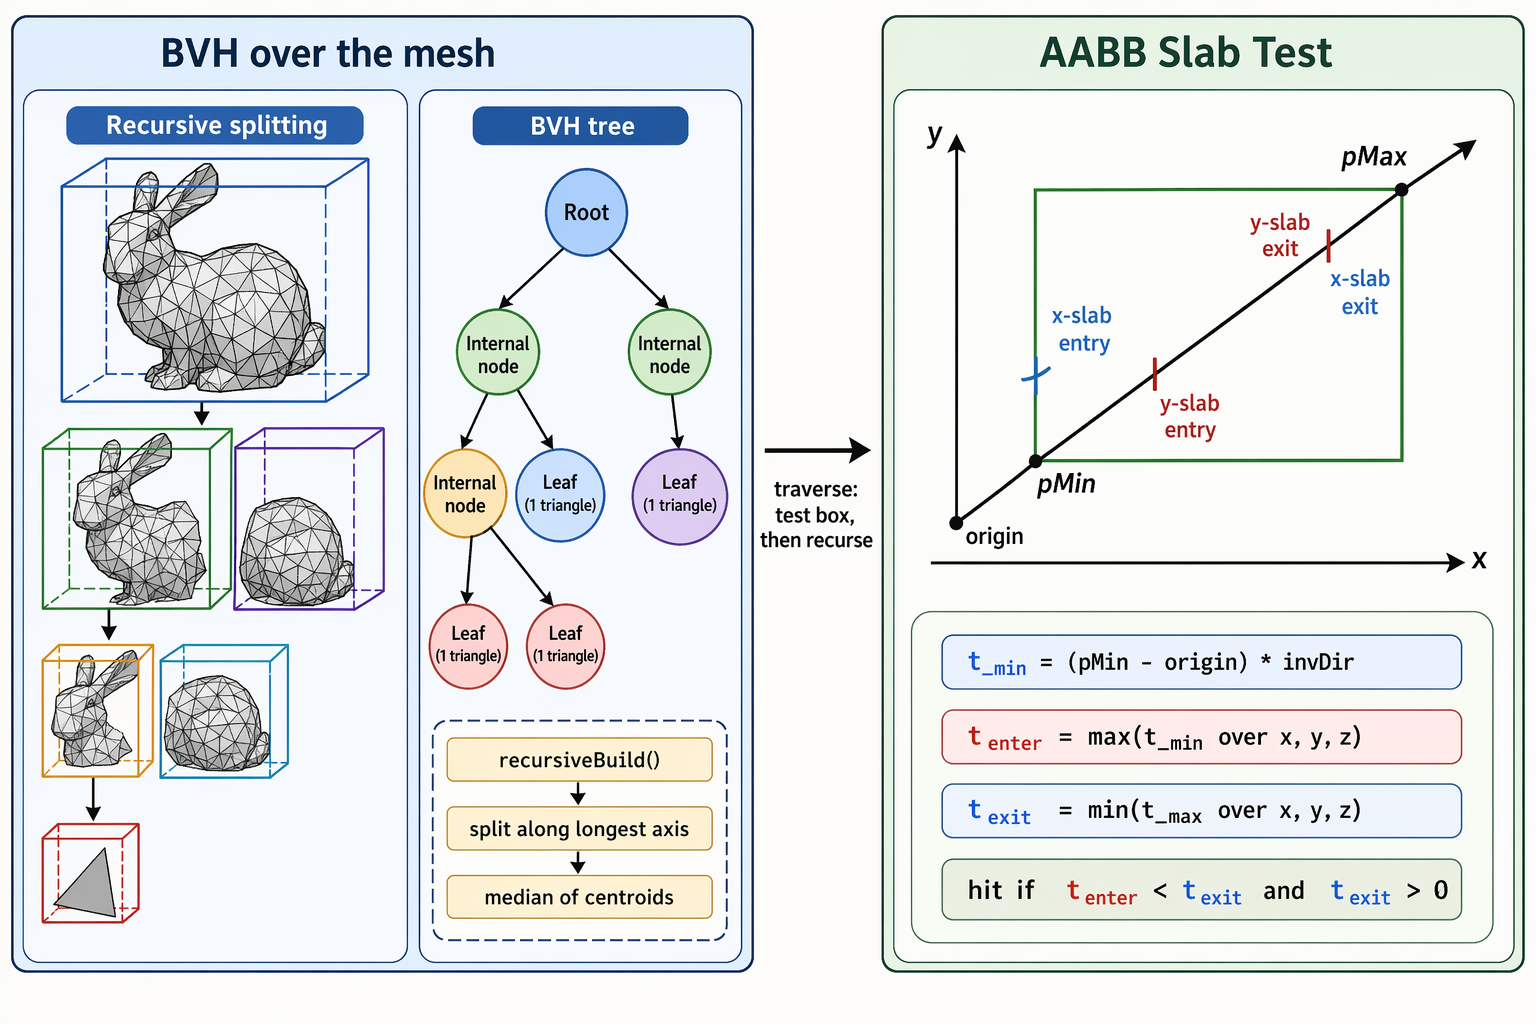
\includegraphics[width=\textwidth]{figures/bvh.png}
  \caption{左：在网格上自顶向下递归构建的 BVH——沿最长轴按质心中位数划分，叶节点对应单个三角形；
  右：AABB slab 求交测试，$t_{\text{enter}}=\max(t^{\min})$、$t_{\text{exit}}=\min(t^{\max})$，
  当 $t_{\text{enter}}<t_{\text{exit}}$ 且 $t_{\text{exit}}>0$ 时命中。}
  \label{fig:bvh}
\end{figure}

\subsection{BVH 遍历求交：\texttt{BVHAccel::getIntersection}}

建立 BVH 后，求交转化为对二叉树的递归遍历：先用 \texttt{IntersectP} 测试当前节点的包围盒，
若不相交则整棵子树都可跳过（剪枝）；若为叶节点则直接与其三角形求交；否则递归左右子树并返回更近的交点。

\begin{lstlisting}
Vector3f invDir(1.0f/ray.direction.x, 1.0f/ray.direction.y, 1.0f/ray.direction.z);
std::array<int,3> dirIsNeg = { int(ray.direction.x > 0),
                               int(ray.direction.y > 0),
                               int(ray.direction.z > 0) };
if (!node->bounds.IntersectP(ray, invDir, dirIsNeg)) return Intersection();   // 剪枝
if (node->left == nullptr && node->right == nullptr)
    return node->object->getIntersection(ray);                                // 叶节点
Intersection hit1 = getIntersection(node->left,  ray);
Intersection hit2 = getIntersection(node->right, ray);
return hit1.distance < hit2.distance ? hit1 : hit2;                            // 取更近者
\end{lstlisting}

\noindent 由于 \texttt{Intersection} 的默认 \texttt{distance} 为 \texttt{double} 最大值，未命中的子树自然
不会赢得最近距离比较，因此无需额外的命中判断即可正确合并左右结果。

\subsection{额外内容：\texttt{castRay\_noBVH} 的完整着色}

框架在检测模式（\texttt{./RayTracing check}）下不会调用 \texttt{buildBVH()}，故 \texttt{scene.bvh} 为空，
原 \texttt{castRay\_noBVH} 仅返回纯白以验证求交是否正确。本部分按文档"额外内容"要求，参照上方的
\texttt{castRay} 补全了完整的 Whitted 着色模型。为不依赖场景级 BVH，新增了暴力最近交点函数：

\begin{lstlisting}
Intersection Scene::intersect_noBVH(const Ray &ray) const {
    Intersection nearest;                       // 默认 distance = DBL_MAX
    for (uint32_t k = 0; k < objects.size(); ++k) {
        Intersection it = objects[k]->getIntersection(ray);
        if (it.happened && it.distance < nearest.distance) nearest = it;
    }
    return nearest;
}
\end{lstlisting}

\noindent \texttt{castRay\_noBVH} 在此基础上完成与 \texttt{castRay} 一致的三分支着色：
（1）反射 + 折射材质用 Fresnel 方程混合反/折射颜色；（2）镜面反射材质追投反射光线；
（3）漫反射/光泽材质使用 Phong 模型（漫反射 + 高光），并对每个光源投射\textbf{阴影光线}判断遮挡：
\begin{equation}
L=\sum_{\text{lights}} (1-\text{inShadow})\,I\,(\mathbf{N}\cdot\mathbf{l})\,k_d\,c_d
   + I\,\max(0,-\mathbf{r}\cdot\mathbf{d})^{p}\,k_s,
\end{equation}
其中阴影测试与递归光线均改用 \texttt{intersect\_noBVH}。Bunny 材质为漫反射/光泽，
故走 Phong 分支，最终检测模式得到与 BVH 模式\textbf{逐像素完全一致}的着色图像。

\section{实验结果}

编译与运行：
\begin{lstlisting}[language=bash,numbers=none]
mkdir build && cd build && cmake .. -DCMAKE_BUILD_TYPE=Release && make
./RayTracing          # BVH 加速渲染 -> binary.ppm
./RayTracing check    # 检测/着色模式 -> binary.ppm
\end{lstlisting}

两种模式的渲染结果如图~\ref{fig:results}。BVH 模式（左）正确渲染出带漫反射与高光、含自阴影的灰色兔子；
检测模式（右）在补全着色模型后得到与之一致的图像，验证了求交与着色逻辑的正确性。

\begin{figure}[H]
  \centering
  \begin{subfigure}{0.49\textwidth}
    \centering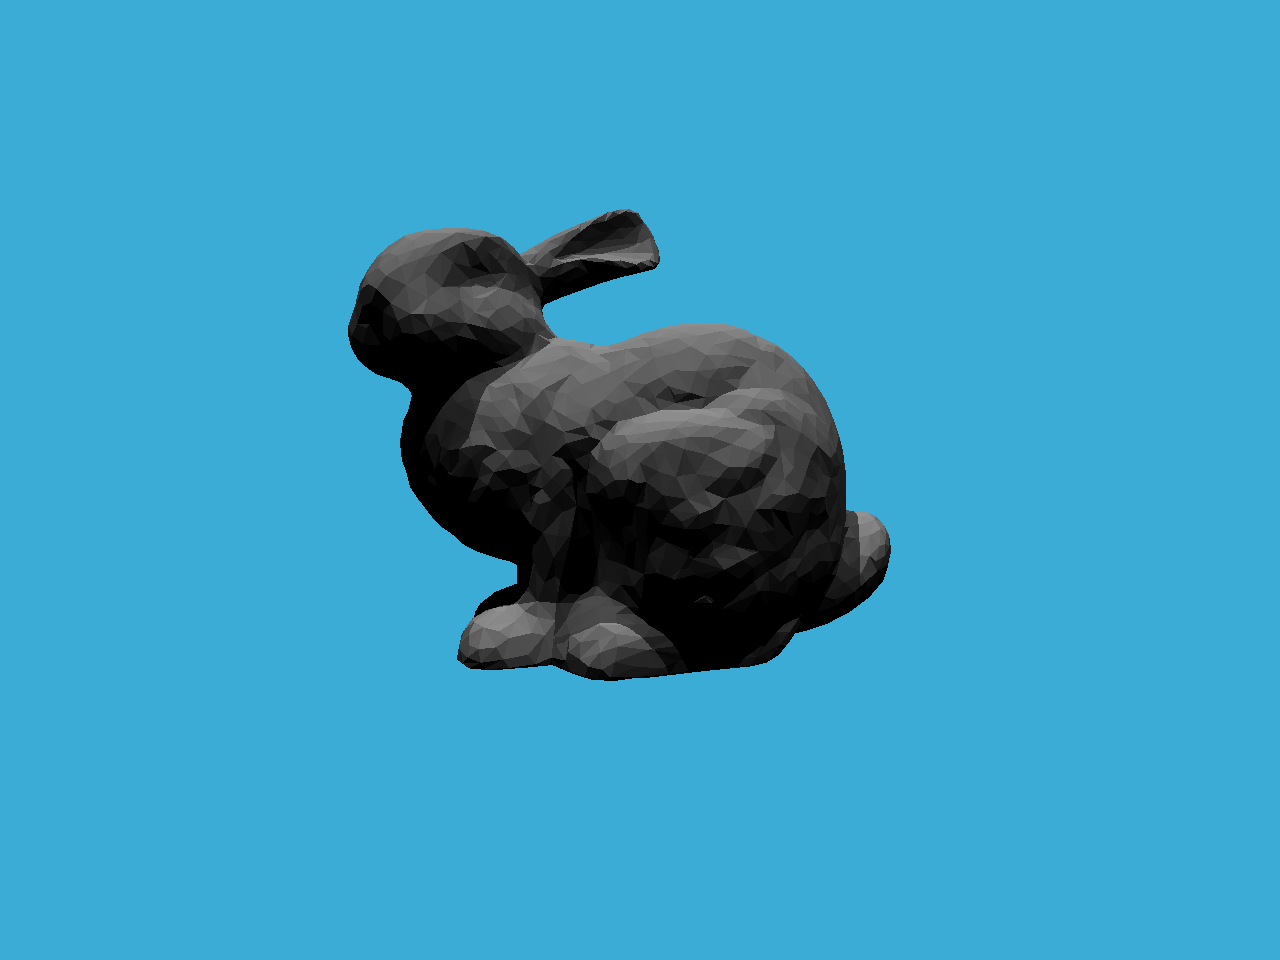
\includegraphics[width=\textwidth]{figures/bunny_bvh.png}
    \caption{BVH 加速渲染（\texttt{./RayTracing}）}
  \end{subfigure}\hfill
  \begin{subfigure}{0.49\textwidth}
    \centering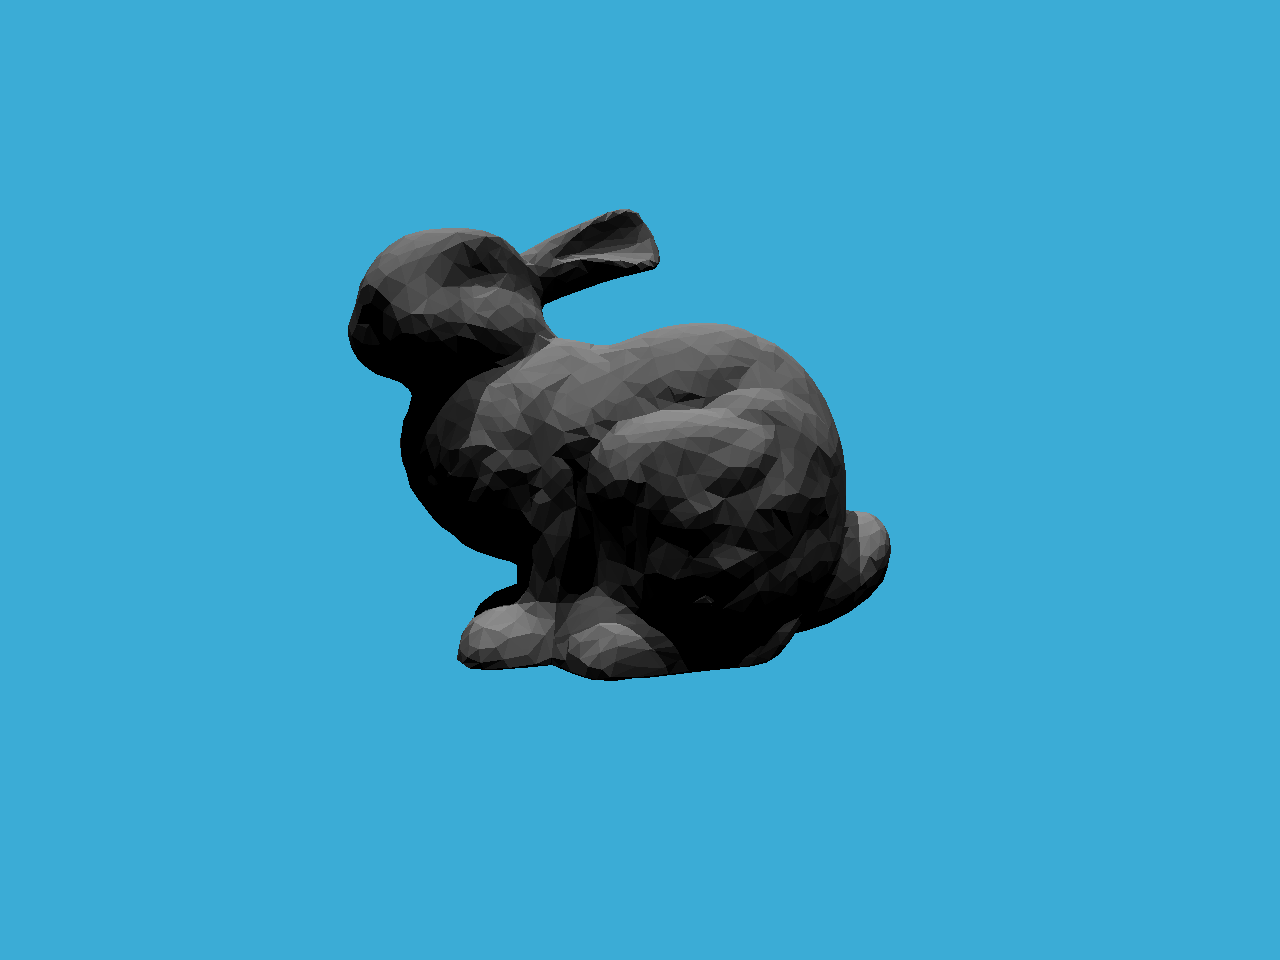
\includegraphics[width=\textwidth]{figures/bunny_check.png}
    \caption{检测/着色模式（\texttt{./RayTracing check}）}
  \end{subfigure}
  \caption{$1280\times960$、4968 三角形的 Stanford Bunny 渲染结果。两图逐像素一致。}
  \label{fig:results}
\end{figure}

本机（release 构建）实测渲染耗时如表~\ref{tab:time}。

\begin{table}[H]
  \centering
  \caption{渲染耗时（4968 三角形，$1280\times960$，3 次取稳定值）}
  \label{tab:time}
  \begin{tabular}{lcc}
    \toprule
    模式 & 是否使用场景级 BVH & 渲染耗时 \\
    \midrule
    \texttt{./RayTracing}        & 是 & $\approx 0.45$\,s \\
    \texttt{./RayTracing check}  & 否（暴力遍历场景物体） & $\approx 0.46$\,s \\
    \bottomrule
  \end{tabular}
\end{table}

\noindent 两者耗时接近，是因为本场景仅含一个网格物体，而 \texttt{MeshTriangle} 在构造时已对其内部
4968 个三角形建立了一层 BVH——即便关闭\textbf{场景级} BVH，网格\textbf{内部}的 BVH 仍在发挥加速作用。
作为对照，文档给出的"完全不使用任何 BVH、逐三角形暴力求交"的参考耗时约为 7 分钟，
而启用 BVH 后降至秒级，凸显了层次包围盒带来的数量级加速。

\section{总结}

本次作业完整实现了基于 BVH 加速的 Whitted 风格光线追踪器：从主光线生成、Möller–Trumbore
光线–三角形求交、AABB slab 包围盒测试，到 BVH 递归遍历，并额外补全了非 BVH 路径下的完整着色模型。
在四千余三角形的 Bunny 场景上以约 0.45\,s 渲染出正确结果。通过本次实践，加深了对光线生成、
解析法求交、空间数据结构加速以及局部光照（Phong + 阴影）等图形学核心概念的理解。

\end{document}
